\chapter{評価}
本章では,全章で提案したヘッドノードにおけるフレーム処理並列化の有効性を確認するため,ヘッドノード内に構築したコンテナ環境において実験を行う.
実験1では,提案手法は既存手法と比較してヘッドノード内でのフレーム処理時間が短縮されているかを確認する.
実験2では,提案手法を用いたマルチディスプレイシステムに対して接続ディスプレイ数を変化させた場合のフレーム処理時間の変化を確認する.
さらに,実験3では,ヘッドノード内で分割コンテナ・圧縮コンテナを動かすにあたり,コンテナの起動と終了に要する時間の測定を行い,コンテナ環境でプロセスを動作させる際のオーバーヘッドについて調べる.
また,実験4では既存手法を用いて構築したマルチディスプレイシステムにおいて全てのノードでコンテナ環境を用意し,完全にコンテナ化されたマルチディスプレイシステムを構築した際のフレームレートについて調査する.
本章では,まず4.1節で,評価で利用した実験環境について説明する.次に,4.2節で,実験1における実験方法と実験結果について述べ,4.3節では,実験2における実験方法と実験結果を述べる.さらに,4.4章では実験3における実験方法と実験結果について述べ,最後に4.5章では実験4に用いた環境とフレームレートの計測結果を示す.

\section{実験環境}
本節では,実験1で用いた実験環境とその方法・結果について述べる.
実験1では,4つのディスプレイを接続して構築した4面構成のマルチディスプレイシステムを想定した実験を行った.
本実験で用いたヘッドノード内のコンテナ構成を図4.2に示す.

当実験環境は,ヘッドノードとして用いるデスクトップPC内のコンテナ仮想環境を用いて構築したものである.
実験環境内では1つの分割コンテナと複数の圧縮コンテナを用意する.
今回の実験では4面構成のディスプレイを想定しているため,ヘッドノード内では1つの分割コンテナと4つの圧縮コンテナを動作させた.

\begin{table}[H]
    \caption{ヘッドノード用デスクトップPCの仕様}
    \begin{center}
    \begin{tabular}{cc}
    \hline
    要素 & 仕様 \\\hline\hline
    CPU & i7-5960X (3.0 GHz×8) \\ \hline
    メモリ & 64.0 GB \\ \hline
    通信帯域 & 1 Gbps \\ \hline
    OS & CentOS 7.3 \\ \hline

    \end{tabular}
    \end{center}
\end{table}

評価に用いる映像としては,クリエイティブ・コモンズ・ライセンスのもとで利用できる3DアニメーションであるBig Buck Bunny \cite{bigbackbunny}を使用した.
表4.4に,Big Buck Bunnyのプロパティを示す.
さらに,図4.3にBig Buck Bunny再生時のスクリーンショットを示す.

\begin{table}[H]
    \caption{Big Buck Bunnyのプロパティ}
    \begin{center}
    \begin{tabular}{cc}
    \hline
    項目 & 内容 \\\hline\hline
    動画形式 & MP4 \\ \hline
    コーデック & H.264 \cite{h264} \\ \hline
    長さ & 10分34秒 \\ \hline
    総フレーム数 & 19020枚 \\ \hline
    フレームレート & 30 fps \\ \hline
    解像度 & 4K (3840×2160) \\ \hline

    \end{tabular}
    \end{center}
\end{table}

\begin{figure}[H]
    \hspace*{\fill}
    \includegraphics[width=\linewidth]{./fig/chap4/bigbuckbunny.eps}
    \hspace*{\fill}
    \caption{Big Buck Bunnyのスクリーンショット}
   \end{figure}

ヘッドノードで行われる処理の実装には,OpenCV \cite{opencv}, libjpeg-turbo ~\cite{libjpeg}, Boost.Asio \cite{asio},gstreamer \cite{gstreamer} という4種類のライブラリを利用した. 
OpenCVは画像処理ライブラリ,libjpeg-turboはJPEGの圧縮と展開を行うライブラリ,Boost.Asioはソケット通信を行うライブラリであり,gstreamerはオープンソースのマルチメディアフレームワークである.
また,ディスプレイノードの処理の実装にはlibjpeg-turbo, Boost.Asio, fbdevを利用した.
実装にはC++言語を使用し,GCCコンパイラ (GNU C Compiler) \cite{gcc}でコンパイルを行った.


\begin{table}[H]
    \caption{評価で利用したソフトウェア}
    \begin{center}
    \begin{tabular}{cc}
    \hline
    ソフトウェア名 & バージョン \\\hline\hline
    OpenCV & 3.4.5/ \\ \hline
    Boost.Asio \cite{h264} & 1.53  \\ \hline
    FFMPEG & 2.8.17 \\ \hline
    libjpeg-turbo & 2.0.1 \\ \hline
    Gstreamer & 1.16.1 \\ \hline
    GCC & 8.5.0 \\ \hline

    \end{tabular}
    \end{center}
\end{table}


\begin{figure}[H]
    \hspace*{\fill}
    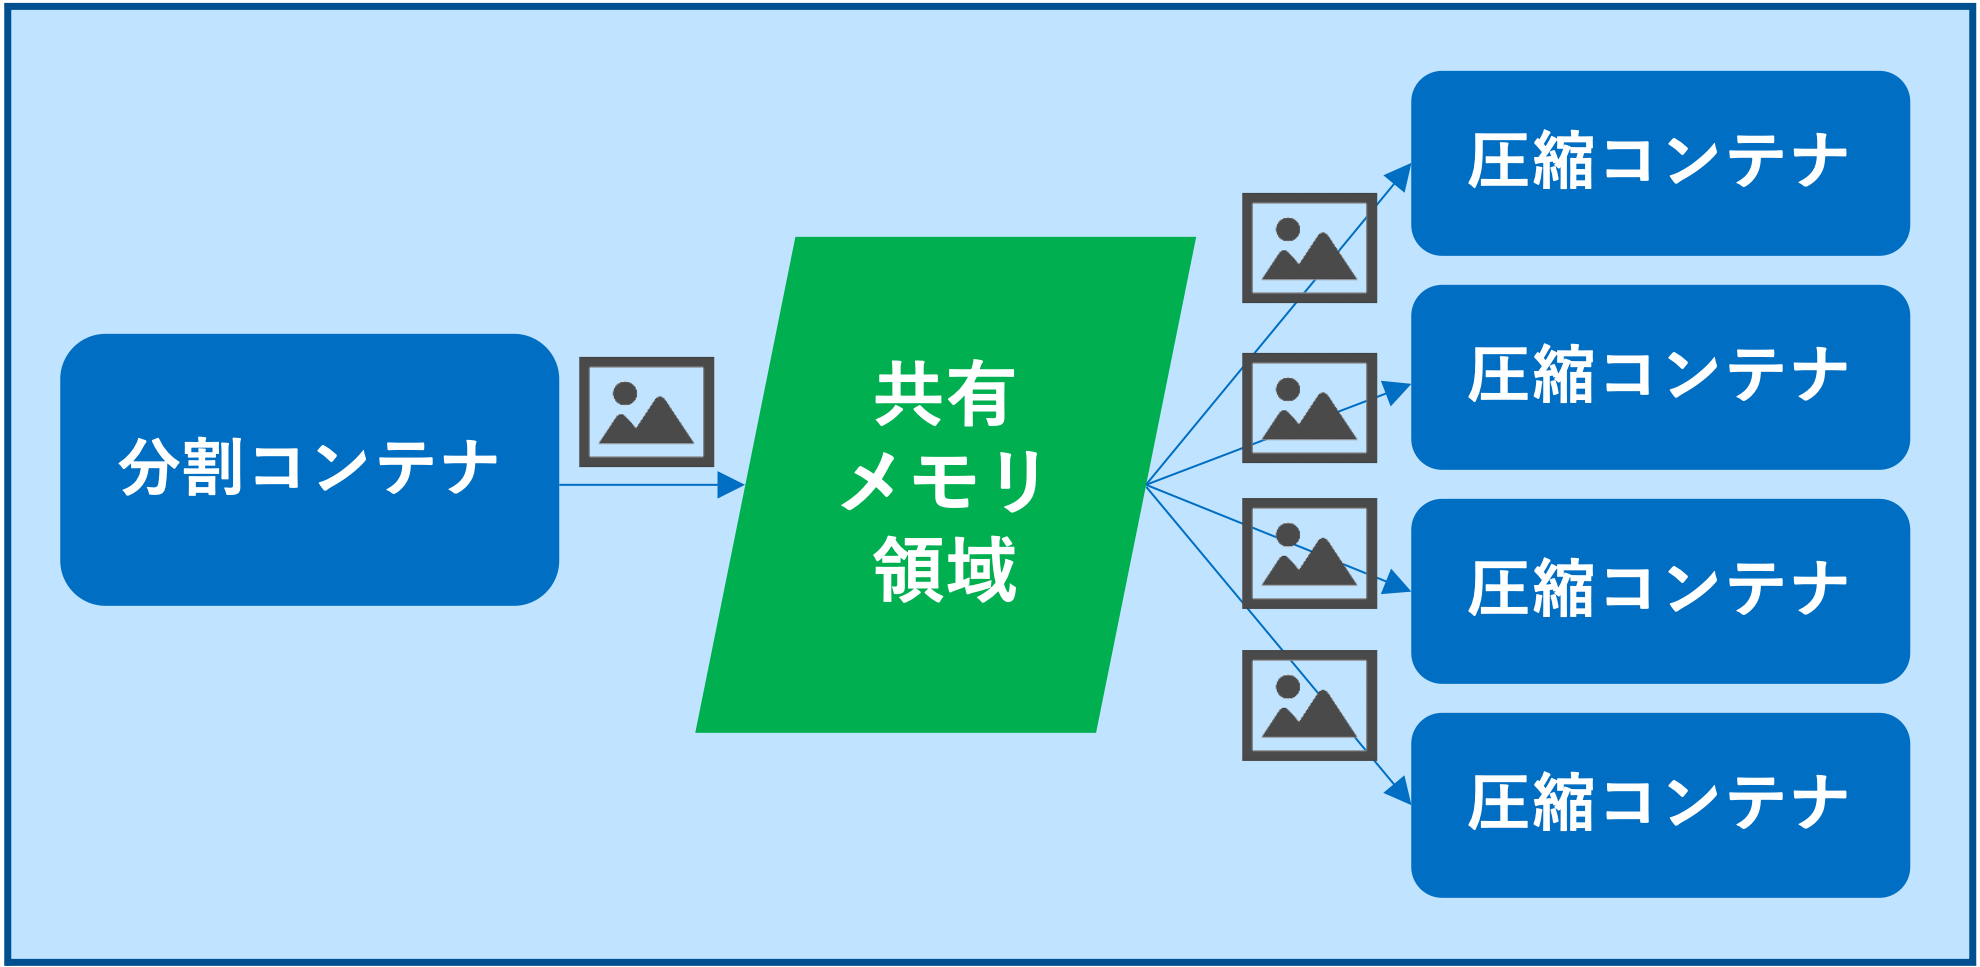
\includegraphics[width=\linewidth]{./fig/chap4/evaluation_environment.eps}
    \hspace*{\fill}
    \caption{実験環境のコンテナ構成}
   \end{figure}

\section{実験1:フレーム処理時間の評価}

\subsection{実験方法}
先行研究で提案された手法と提案手法において,4面構成のMDを想定した環境で4K解像度の画像を表示し,動画のフレーム開始から1000フレーム目の処理が終了するまでの1フレームあたりに要するフレーム処理時間を計測した.
また,フレーム処理時間の計測にはC++11の時間ライブラリであるchronoを用いた.

\subsection{実験結果}
図xxxに先行研究で提案されたシステムと提案手法でのフレーム処理時間を示す.
既存手法においてフレームの処理に要する時間の平均を計測すると,それぞれ拡大・分割に5.04ms, 圧縮には47.31msであった.
結果より,フレームの拡大と分割に比べてフレームの圧縮に長い時間がかかっている事がわかる.
また,1フレームあたりに要する処理時間は拡大・分割にかかる時間と圧縮にかかる時間との和で表すことができ,その時間は52.35msとなる.
1フレームあたりの処理時間を用いることで1秒あたりに何フレームを表示する事ができるかを示す動作時フレームレートを計算する事ができる.
この場合では,動作時フレームレートは1000/52.35 ≒ 19.1[fps]となり,この付近に動作時フレームレートの限界があることがわかる.

一方提案手法においてフレームの処理に要する時間の平均を計測すると,それぞれ拡大・分割に4.82ms, 共有メモリへの格納に0.77ms, 共有メモリからの取り出しに0.02ms, 圧縮には16.11msであった.フレームの拡大.分割については既存手法と提案手法とで処理に差はないため,既存手法と同等の処理時間を要している.
フレームの圧縮処理においては,OS仮想化技術を用いた並列化の効果が顕著に現れており,既存手法と比較しておよそ3分の1程度の時間で行う事が可能となっている.
さらに,フレーム圧縮処理を並列化することによって生じたオーバーヘッドである共有メモリを用いたプロセス間でのフレーム受け渡し処理においても,1ms未満の非常に短い時間で行えている事がわかる.
これは,ホストマシン内のメモリ領域に対してはコンテナ内からmemcpy()関数を用いた高速なデータ書き込み/読み出しが可能であることを表している.
また,全体のフレーム処理時間について比較すると,提案手法では既存手法から60\%程度短縮することに成功している.
以上の結果より,フレーム処理プロセスの並列化を行った提案手法によって,システムのボトルネックが解消されたことが確認できる.

\begin{figure}[H]
    \hspace*{\fill}
    \includegraphics[width=\linewidth]{./fig/chap4/processing_time_4.eps}
    \hspace*{\fill}
    \caption{フレーム処理時間の比較 (4面構成時)}
\end{figure}


\section{実験2:スケーラビリティに関する評価}
実験2では,構成ディスプレイ数を増加させた場合におけるフレーム処理時間の変化を調べる.
本実験では,ディスプレイ9面構成のマルチディスプレイを構築することを想定し,実験1の結果との比較を行う.
本実験のヘッドノード内では,1つの分割コンテナと9つの圧縮コンテナを動作させる.

 \subsection*{実験結果}
 図xxxに先行研究で提案されたシステムと提案手法における,9面構成のマルチディスプレイを想定した場合のフレーム処理時間を示す.
 また,比較のために4面構成のディスプレイを想定した,実験1の計測結果も再掲している.

\begin{figure}[H]
    \hspace*{\fill}
    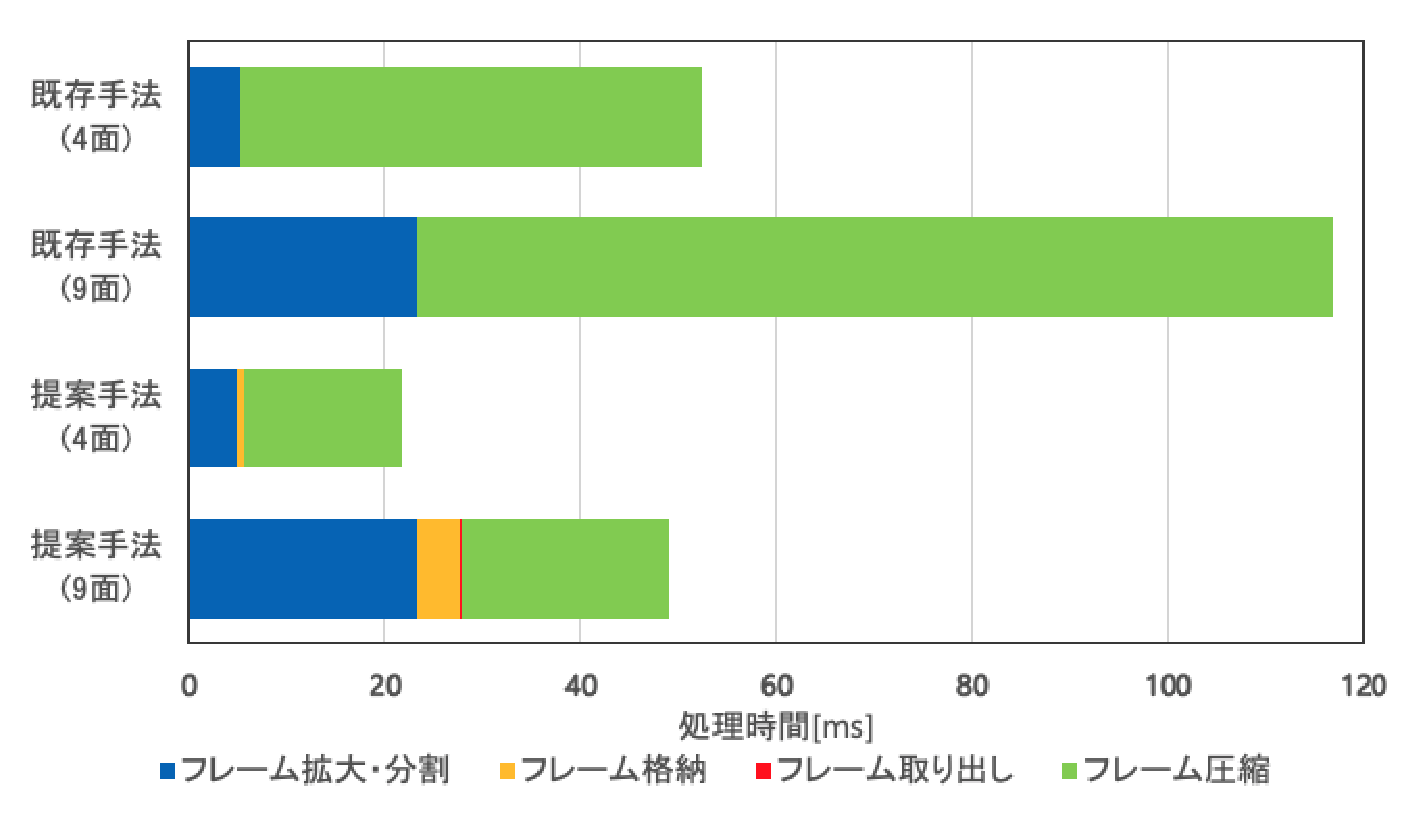
\includegraphics[width=\linewidth]{./fig/chap4/processing_time_49.eps}
    \hspace*{\fill}
    \caption{フレーム処理時間の比較 (9面構成時)}
\end{figure}


\section{コンテナの起動時間に関する評価}
本節では,

\section{CPU使用率に関する評価}
\section{MDのコンテナ化の評価}
本節では,マルチディスプレイシステムのコンテナ化を行った実験について記す.
本実験は,先行研究において提案された,SBCマルチディスプレイシステムの完全なコンテナ仮想化についての可能性を探るためのものである.
マルチディスプレイシステムを構成する各ノードに仮想化環境を導入し,その環境上で各ノードのプロセスを動作させることにより,異なるSBCをディスプレイノードとして使用した場合にもアーキテクチャ・仕様の差異を吸収して同一の環境で動作させることが可能となる.
本実験では,SBCの一種であり,Dockerが標準的にサポートされているJetson Nano \cite{jetson}をディスプレイノードとして使用し,仮想環境上でノードプロセスを動作させた場合におけるマルチディスプレイシステム全体のパフォーマンスを計測した.

\subsection*{実験環境}
実験4に用いた実験兼環境について説明する.
ヘッドノードは実験1で用いたもののと同様のものを使用している.
ディスプレイノードにはSBCの一種であるJetson Nanoを用いた.
図xxxにJetson Nanoの画像を,表xxxに仕様を示す.

\begin{figure}[H]
    \hspace*{\fill}
    \includegraphics[width=60mm]{./fig/chap4/jetson.eps}
    \hspace*{\fill}
    \caption{Jetson Nano}
\end{figure}

\begin{table}[H]
    \caption{Jetson Nanoの仕様}
    \begin{center}
    \begin{tabular}{cc}
    \hline
    要素 & 仕様 \\\hline\hline
    CPU & ARM Cortex-A57(4コア/1.43GHz) \\ \hline
    GPU & CUDAコア128基/Maxwellアーキテクチャ/472GFLOPS \\ \hline
    メモリ & 4GB/64bit LPDDR4 \\ \hline
    OS & Jetson Nano Developer Kit(Ubuntu 18.04 LTS)\\ \hline

    \end{tabular}
    \end{center}
\end{table}

実験の際にはJetson Nano4台をディスプレイノードとして使用し,ディスプレイ4面構成のマルチディスプレイシステムを構築した.
ヘッドノードとディスプレイノード群の間には1台のイーサネットスイッチ (1Gbps)が接続されている.
本実験で用いた評価環境の図を図4.2に示す.

\begin{figure}[H]
    \hspace*{\fill}
    \includegraphics[width=\linewidth]{./fig/chap4/jikken4.eps}
    \hspace*{\fill}
    \caption{実験4で用いた実験環境}
\end{figure}

なお,評価に用いた映像,ソフトウェアなどは全て実験1と同様のものである.

\subsection*{実験方法}
4面構成のマルチディスプレイにおいて,先行研究で提案されたミドルウェアをヘッドノード,ディスプレイノードそれぞれに構築した仮想環境上で
動作させ,動画表示のフレームレートを計測した.
また,動作時の目標フレームレートは動画本来のフレームレートである30fpsに設定した.

\subsection*{実験結果}
図xxxに,仮想環境上において先行研究で提案されたミドルウェアを動作させた場合のフレームレートの時間変化を示す.

\begin{figure}[H]
    \hspace*{\fill}
    \includegraphics[width=\linewidth]{./fig/chap4/framerate_docker.eps}
    \hspace*{\fill}
    \caption{フレームレートの時間変化}
\end{figure}

実験の結果,マルチディスプレイ上に4K解像度の映像を表示した場合におけるフレームレートの平均値は,22.55fpsであった.
この結果から,各ノードを仮想化環境上で構築した際においても,動作時のフレームレートは大きく変化していない事が確認できた.

\subsection*{結果に対する考察}